\documentclass[12pt]{article}
\usepackage[margin=1in]{geometry} 
\usepackage{amsmath,amsthm,amssymb,amsfonts}
\usepackage{tabto}
\usepackage{hyperref}

\usepackage{arydshln} % gives hdashline and cdashline
\newcommand*{\tempb}{\multicolumn{1}{:c}{}} % Used for block matrices

% Spacers:
% BEGIN BLOCK------------------------------------------
% END BLOCK============================================




\newcommand{\N}{\mathbb{N}}
\newcommand{\Z}{\mathbb{Z}}

% CUSTOM SETTINGS
% BEGIN BLOCK------------------------------------------
% For equation system alignment
\usepackage{systeme,mathtools}
% Usage:
%	\[
%	\sysdelim.\}\systeme{
%	3z +y = 10,
%	x + y +  z = 6,
%	3y - z = 13}


% For definitions
\newtheorem{defn}{Definition}[section]
\newtheorem{thrm}{Theorem}[section]

% For circled text
\usepackage{tikz}
\usetikzlibrary{matrix}
\newcommand*\circled[1]{\tikz[baseline=(char.base)]{
            \node[shape=circle,draw,inner sep=0.8pt] (char) {#1};}}

\newenvironment{problem}[2][Problem]{\begin{trivlist}
\item[\hskip \labelsep {\bfseries #1}\hskip \labelsep {\bfseries #2.}]}{\end{trivlist}}
%If you want to title your bold things something different just make another thing exactly like this but replace "problem" with the name of the thing you want, like theorem or lemma or whatever
 
%used for matrix vertical line
\makeatletter
\renewcommand*\env@matrix[1][*\c@MaxMatrixCols c]{%
  \hskip -\arraycolsep
  \let\@ifnextchar\new@ifnextchar
  \array{#1}}
\makeatother 

% END BLOCK============================================

\newtheorem*{lemma}{Lemma} %added
\newtheorem*{result}{Result} %added
\newtheorem*{theorem}{Theorem} %added
\theoremstyle{definition}
\newtheorem*{solution}{Solution} %added
\theoremstyle{plain}

% HEADER
% BEGIN BLOCK------------------------------------------
\usepackage{fancyhdr}
 
\pagestyle{fancy}
\fancyhf{}
\lhead{Homework \#14}
\rhead{Bryan Greener}
\cfoot{\thepage}
% END BLOCK============================================

% TITLE
% BEGIN BLOCK------------------------------------------
\title{Bryan Greener}
\author{MATH 2300 CRN:15163}
\date{2018-04-10}
\begin{document}
\maketitle
% END BLOCK============================================

\TabPositions{4cm}

\begin{enumerate}
\item[11.71]Find the characteristic and minimum polynomials of each matrix:
	\begin{enumerate}
	\item $A=\begin{bmatrix}[rrr]3&1&-1\\2&4&-2\\-1&-1&3\\\end{bmatrix}$\\
	\[ A-\lambda I = \begin{bmatrix}[rrr]3-\lambda & 1 & -1\\2&4-\lambda &-2\\-1&-1&3-\lambda\\\end{bmatrix} \]
	Next we compute the determinant
	\[ \mathrm{det}(A) = -\lambda^3+10\lambda^2-28\lambda+24 = (\lambda-6)(\lambda-2)^2 \]
	Thus $m(t)$ is either $f(t)=(t-6)(t-2)$ or $g(t)=(t-6)(t-2)^2$.\\
	By the Cayley-Hamilton theorem, $g(A)=\Delta(A)=0$. Hence we only need to test $f(t)$.
	\[ f(A)=(A-6I)(A-2I) = \begin{bmatrix}[rrr]-3&1&-1\\2&-2&-2\\-1&-1&-3\\\end{bmatrix}\begin{bmatrix}[rrr]1&1&-1\\2&2&-2\\-1&-1&1\\\end{bmatrix} = \begin{bmatrix}[rrr]0&0&0\\0&0&0\\0&0&0\\\end{bmatrix} \]
	Thus $m(t)=f(t)=(t-6)(t-2)=t^2-12t+12$ is the minimal polynomial of $A$.
	
	\item $B=\begin{bmatrix}[rrr]3&2&-1\\3&8&-3\\3&6&-1\\\end{bmatrix}$\\
	Repeating the process from part (a), we get $\mathrm{det}(B)=-\lambda^3+10\lambda^2-28\lambda+24$. Since this is the same characteristic polynomial as part (a), then we get the same set of possibilities for $m(t)$. Thus we only need to test
	\[ \begin{bmatrix}[rrr]3&2&-1\\3&8&-3\\3&6&-1\\\end{bmatrix}\begin{bmatrix}[rrr]1&2&-1\\3&6&-3\\3&6&-3\\\end{bmatrix}\neq\begin{bmatrix}[rrr]0&0&0\\0&0&0\\0&0&0\\\end{bmatrix} \]
	Since $m(t)\neq f(t)$, then $m(t)=g(t)=(t-6)(t-2)^2$.
	\end{enumerate}
\item[11.72]Find the characteristic and minimum polynomials of each matrix:
	\begin{enumerate}
	\item $A=\begin{bmatrix}[rrrrr]2&5&0&0&0\\0&2&0&0&0\\0&0&4&2&0\\0&0&3&5&0\\0&0&0&0&7\\\end{bmatrix}$\\
	This matrix is block diagonal with blocks
	\[ A=\begin{bmatrix}[rr]2&5\\0&2\\\end{bmatrix}, \quad B=\begin{bmatrix}[rrr]4&2\\3&5\\\end{bmatrix}, \quad C=\begin{bmatrix}[r]7\\\end{bmatrix} \]
	The matrix $A$ has minimum polynomial of $f(t)=(t-2)^2$ and $B$ has $g(t)=(t-2)(t-7)$ and $C$ has $h(t)=(t-7)$. Thus $\Delta(t) = f(t)g(t)h(t) = (t-2)^3(t-7)^2$. So $m(t)=LCM[f(t)g(t)h(t)] = (t-2)^2(t-7)$.
	\item $B=\begin{bmatrix}[rrrrr]4&-1&0&0&0\\1&2&0&0&0\\0&0&3&1&0\\0&0&0&3&1\\0&0&0&0&3\\\end{bmatrix}$\\
	This matrix has the block matrices
	\[ A=\begin{bmatrix}[rr]4&-1\\1&2\\\end{bmatrix}, \quad B=\begin{bmatrix}[rrr]3&1&0\\0&3&1\\0&0&3\\\end{bmatrix} \]
	$A$ has minimum polynomial $f(t)=(t-3)^2$ and $B$ has $g(t)=(t-3)^3$. Thus $\Delta(t)=(t-3)^5$ but $m(t)=(t-3)^3$.
	\item $C=\begin{bmatrix}[rrrrr]3&2&0&0&0\\1&4&0&0&0\\0&0&3&1&0\\0&0&1&3&0\\0&0&0&0&4\\\end{bmatrix}$\\
	This matrix has the block matrices
	\[ A=\begin{bmatrix}[rr]3&2\\1&4\\\end{bmatrix}, \quad B=\begin{bmatrix}[rrr]3&1&0\\1&3&0\\0&0&4\\\end{bmatrix}, \quad C=\begin{bmatrix}[r]4\\\end{bmatrix} \]
	Matrix $A$ has the minimum polynomial $f(t)=(t-2)(t-5)$ and $B$ has $g(t)=(t-4)(t-2)$ and $C$ has $h(t)=(t-4)$. Thus $\Delta(t)=(t-2)^2(t-5)(t-4)^2$ but $m(t)=(t-2)(t-4)(t-5)$.
	\end{enumerate}
\item[11.75]Show that a matrix $A$ and its transpose $A^T$ have the same minimum polynomial.\\
	

\item[11.77]Show that $A$ is a scalar matrix $kI$ if and only if the minimum polynomial of $A$ is $m(t)=t-k$.
\begin{proof}
Let $A$ be a scalar matrix $kI$. We show that this leads to $m(t)=(t-k)$.\\
Then 
\[ A=\begin{bmatrix}[rrrr]
k&0&\cdots&0\\
0&k&\cdots&0\\
\vdots&\vdots&\ddots&\vdots\\
0&0&\cdots&k\\\end{bmatrix} \]
Thus the characteristic polynomial of this $n\times n$ matrix is $\Delta(t) = (t-k)^n$. However since every element in the diagonal is $k$ then the minimum polynomial is $m(t) = (t-k)$.\\
Next let $m(t)=(t-k)$ for some matrix $A$. We show that this leads to $A = kI$. Then the characteristic polynomial of $A$ must be able to factor into some degree of $\Delta(t)=(t-k)^m$ where $m$ is an unknown degree. Since the only item in our minimum polynomial is $(t-k)$, then the only nonzero items in the diagonal of $A$ are $k$. Therefore the original matrix must be
\[ A=\begin{bmatrix}[rrrr]
k&0&\cdots&0\\
0&k&\cdots&0\\
\vdots&\vdots&\ddots&\vdots\\
0&0&\cdots&k\\\end{bmatrix} \]
which can be rewritten as $A=kI$.
\end{proof}
\item[11.78]Find a matrix $A$ whose minimum polynomial is: (a) $t^3-5t^2+6t+8$; (b) $t^4-5t^3-2t+7t+4$.
	\begin{enumerate}
	\item $A=\begin{bmatrix}[rrr]0&0&-8\\1&0&-6\\0&1&5\\\end{bmatrix}$
	\item $A=\begin{bmatrix}[rrrr]0&0&0&-4\\1&0&0&-7\\0&1&0&2\\0&0&1&5\\\end{bmatrix}$
	\end{enumerate}
\item[11.79]Consider the following matrices in Jordan canonical form:
\[ A=\begin{bmatrix}[ccccccccccc]
	4&1&0&\tempb &{}&{}&{}&{}&{}&{}&{}\\
	0&4&1&\tempb &{}&{}&{}&{}&{}&{}&{}\\
	0&0&4&\tempb &{}&{}&{}&{}&{}&{}&{}\\
	\cdashline{1-6}
	{}&{}&{}&\tempb &4&1&\tempb &{}&{}&{}&{}\\
	{}&{}&{}&\tempb &0&4&\tempb &{}&{}&{}&{}\\
	\cdashline{4-9}
	{}&{}&{}&{}&{}&{}&\tempb &2&1&\tempb &{}\\
	{}&{}&{}&{}&{}&{}&\tempb &0&2&\tempb &{}\\
	\cdashline{7-11}
	{}&{}&{}&{}&{}&{}&{}&{}&{}&\tempb &2\\\end{bmatrix} 
	\quad B=\begin{bmatrix}[ccccccccccc]
	4&1&\tempb &{}&{}&{}&{}&{}&{}&{}&{}\\
	0&4&\tempb &{}&{}&{}&{}&{}&{}&{}&{}\\
	\cdashline{1-5}
	{}&{}&\tempb &4&1&\tempb &{}&{}&{}&{}&{}\\
	{}&{}&\tempb &0&4&\tempb &{}&{}&{}&{}&{}\\
	\cdashline{3-7}
	{}&{}&{}&{}&{}&\tempb &4 &\tempb &{}&{}&{}\\
	\cdashline{6-11}	
	{}&{}&{}&{}&{}&{}&{}&\tempb &2&1&0\\	
	{}&{}&{}&{}&{}&{}&{}&\tempb &0&2&1\\	
	{}&{}&{}&{}&{}&{}&{}&\tempb &0&0&2\\\end{bmatrix}	
	\]
	\begin{enumerate}
	\item Find the characteristic polynomials of $A$ and $B$.\\
	Since both matrices have five 4s and three 2s on the diagonal, then $\Delta(t)=(t-4)^5(t-2)^3$ is the characteristic polynomial of both $A$ and $B$ and their eigenvalues are 2 and 4.
	\item Find the minimum polynomials of $A$ and $B$.\\
	The minimum polynomial for $A$ is $(t-4)^3(t-2)^2$ since the largest block with 4s in the diagonal is of order 3 and the largest block with 2s is of order 2. The minimum polynomial for $B$ is $(t-4)^2(t-2)^3$ for the opposite reason of A's minimum polynomial.
	\item Find a maximal set $S$ of linearly independent eigenvectors of $A$.\\
	Since each block contributes one eigenvector to $S$, then a maximal set can be $v_1=(1,0,0,0,0,0,0,0),v_2=(0,0,0,1,0,0,0,0),v_3=(0,0,0,0,0,1,0,0),v_4=(0,0,0,0,0,0,0,1)$.
	\item Find a maximal set $S$ of linearly independent eigenvectors of $B$.\\
	Since each block contributes one eigenvector to $S$, then a maximal set can be $v_1=(1,0,0,0,0,0,0,0),v_2=(0,0,1,0,0,0,0,0),v_3=(0,0,0,0,1,0,0,0),v_4=(0,0,0,0,0,1,0,0)$.
	\end{enumerate}
	
\item[11.80]Find all possible Jordan canonical forms whose characteristic polynomials $\Delta (t)$ and minimum polynomials $m(t)$ are as follows: (a) $\Delta (t)=(t-2)^4(t-3)^2,m(t)=(t-2)^2(t-3)^2$; (b) $\Delta (t)=(t-7)^5,m(t)=(t-7)^2$; (c) $\Delta (t) =(t-8)^4(t-1)^3,m(t)=(t-8)^3(t-1)^2$.
	\begin{enumerate}
	\item 
	\[ \begin{bmatrix}[cccccccc]
	2&1&\tempb&{}&{}&{}&{}&{}\\
	0&2&\tempb&{}&{}&{}&{}&{}\\
	\cdashline{1-5} 
	{}&{}&\tempb&2&1&\tempb&{}&{}\\
	{}&{}&\tempb&0&2&\tempb&{}&{}\\
	\cdashline{3-8} 
	{}&{}&{}&{}&{}&\tempb&3&1\\
	{}&{}&{}&{}&{}&\tempb&0&3\\
	\end{bmatrix}, \quad \begin{bmatrix}[ccccccccc]
	2&1&\tempb&{}&{}&{}&{}&{}&{}\\
	0&2&\tempb&{}&{}&{}&{}&{}&{}\\
	\cdashline{1-4}
	{}&{}&\tempb&2&\tempb&{}&{}&{}&{}\\
	\cdashline{3-6}
	{}&{}&{}&{}&\tempb&2&\tempb&{}&{}\\
	\cdashline{5-9}
	{}&{}&{}&{}&{}&{}&\tempb&3&1\\
	{}&{}&{}&{}&{}&{}&\tempb&0&1\\\end{bmatrix} \]
	\item
	\[ \begin{bmatrix}[ccccccc]
	7&1&\tempb&{}&{}&{}&{}\\
	0&7&\tempb&{}&{}&{}&{}\\
	\cdashline{1-5}
	{}&{}&\tempb&7&1&\tempb&{}\\
	{}&{}&\tempb&0&7&\tempb&{}\\
	\cdashline{3-7}
	{}&{}&{}&{}&{}&\tempb&7\\\end{bmatrix}, \quad
	\begin{bmatrix}[cccccccc]
	7&1&\tempb&{}&{}&{}&{}&{}\\
	0&7&\tempb&{}&{}&{}&{}&{}\\
	\cdashline{1-4}
	{}&{}&\tempb&7&\tempb&{}&{}&{}\\
	\cdashline{3-6}
	{}&{}&{}&{}&\tempb&7&\tempb&{}\\
	\cdashline{5-8}
	{}&{}&{}&{}&{}&{}&\tempb&7\\\end{bmatrix} \]

	\item Trying a different method of drawing these pictures using tikzpicture.\\
	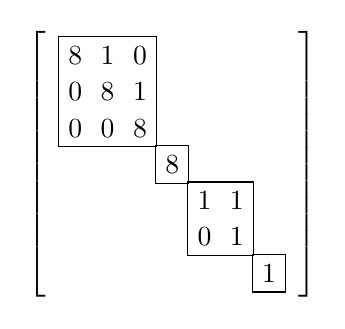
\begin{tikzpicture}
		\matrix(m)[
			matrix of math nodes,
			nodes in empty cells,
			left delimiter={[},
			right delimiter={]}]{
			8&1&0&{}&{}&{}&{}\\
			0&8&1&{}&{}&{}&{}\\
			0&0&8&{}&{}&{}&{}\\
			{}&{}&{}&8&{}&{}&{}\\
			{}&{}&{}&{}&1&1&{}\\
			{}&{}&{}&{}&0&1&{}\\
			{}&{}&{}&{}&{}&{}&1\\
			};
		\draw (m-3-1.south west) rectangle (m-1-3.north east);
		\draw (m-4-4.south west) rectangle (m-4-4.north east);
		\draw (m-6-5.south west) rectangle (m-5-6.north east);
		\draw (m-7-7.south west) rectangle (m-7-7.north east);
	\end{tikzpicture}
	\end{enumerate}		
\item[11.81]The six possible Jordan canonical forms with characteristic polynomial $\Delta (t)=(t-2)^3(t-5)^2$ follow:\\
\[B_1=\begin{bmatrix}[cccccc]
2&1&0&\tempb&{}&{}\\
0&2&1&\tempb&{}&{}\\
0&0&2&\tempb&{}&{}\\
\cdashline{1-6}
{}&{}&{}&\tempb&5&1\\
{}&{}&{}&\tempb&0&5\\\end{bmatrix}
,\quad 
B_2=\begin{bmatrix}[ccccccc]
2&1&\tempb&{}&{}&{}&{}\\
0&2&\tempb&{}&{}&{}&{}\\
\cdashline{1-4}
{}&{}&\tempb&2&\tempb&{}&{}\\
\cdashline{3-7}
{}&{}&{}&{}&\tempb&5&1\\
{}&{}&{}&{}&\tempb&0&5\\\end{bmatrix} \]
\[ B_3=\begin{bmatrix}[cccccccc]
2&\tempb&{}&{}&{}&{}&{}&{}\\
\cdashline{1-3}
{}&\tempb&2&\tempb&{}&{}&{}&{}\\
\cdashline{2-5}
{}&{}&{}&\tempb&2&\tempb&{}&{}\\
\cdashline{4-8}
{}&{}&{}&{}&{}&\tempb&5&1\\
{}&{}&{}&{}&{}&\tempb&0&5\\\end{bmatrix}
,\quad
B_4=\begin{bmatrix}[ccccccc]
2&1&0&\tempb&{}&{}&{}\\
0&2&1&\tempb&{}&{}&{}\\
0&0&2&\tempb&{}&{}&{}\\
\cdashline{1-5}
{}&{}&{}&\tempb&5&\tempb&{}\\
\cdashline{4-7}
{}&{}&{}&{}&{}&\tempb&5\\\end{bmatrix}\]
\[ B_5=\begin{bmatrix}[cccccccc]
2&1&\tempb&{}&{}&{}&{}&{}\\
0&2&\tempb&{}&{}&{}&{}&{}\\
\cdashline{1-4}
{}&{}&\tempb&2&\tempb&{}&{}&{}\\
\cdashline{3-6}
{}&{}&{}&{}&\tempb&5&\tempb&{}\\
\cdashline{5-8}
{}&{}&{}&{}&{}&{}&\tempb&5\\\end{bmatrix}
,\quad
B_6=\begin{bmatrix}[ccccccccc]
2&\tempb&{}&{}&{}&{}&{}&{}&{}\\
\cdashline{1-3}
{}&\tempb&2&\tempb&{}&{}&{}&{}&{}\\
\cdashline{2-5}
{}&{}&{}&\tempb&2&\tempb&{}&{}&{}\\
\cdashline{4-7}
{}&{}&{}&{}&{}&\tempb&5&\tempb&{}\\
\cdashline{6-9}
{}&{}&{}&{}&{}&{}&{}&\tempb&5\\\end{bmatrix} \]
In each case, find the minimum polynomial m(t) and a maximal set $S$ of linearly independent eigenvectors.
	\begin{solution} Minimal polynomials:
	\[ B_1:m(t)=(t-2)^3(t-5)^2,\quad B_2:m(t)=(t-2)^2(t-5)^2,\quad B_3:m(t)=(t-2)(t-5)^2 \]
	\[ B_4:m(t)=(t-2)^2(t-5),\quad B_5:m(t)=(t-2)^2(t-5),\quad B_6:m(t)=(t-2)(t-5) \]
	Next we find the maximal set $S$ of linearly independent eigenvectors.
	\begin{align*}
	B_1:& v_1=(1,0,0,0,0),v_2=(0,0,0,1,0)\\
	B_2:& v_1=(1,0,0,0,0),v_2=(0,0,1,0,0),v_3=(0,0,0,1,0)\\
	B_3:& v_1=(1,0,0,0,0),v_2=(0,1,0,0,0),v_3=(0,0,1,0,0),v_4=(0,0,0,1,0)\\
	B_4:& v_1=(1,0,0,0,0),v_2=(0,0,0,1,0),v_3=(0,0,0,0,1)\\
	B_5:& v_1=(1,0,0,0,0),v_2=(0,0,1,0,0),v_3=(0,0,0,1,0),v_4=(0,0,0,0,1)\\
	B_6:& v_1=(1,0,0,0,0),v_2=(0,1,0,0,0),v_3=(0,0,1,0,0),v_4=(0,0,0,1,0),v_5=(0,0,0,0,1)
	\end{align*}
	\end{solution}
	
\item[12.28]For each matrix $A$, find a nonsingular matrix $P$ and a diagonal matrix $D$ such that $D=P^TAP$:
	\begin{enumerate}
	\item $A=\begin{bmatrix}[rrr]1&0&2\\0&3&6\\2&6&7\\\end{bmatrix}$\\
	We start by diagonalizing $A$.
	\begin{align*}
	M=[A,I]&= \begin{bmatrix}[rrr|rrr]1&0&2&1&0&0\\0&3&6&0&1&0\\2&6&7&0&0&1\\\end{bmatrix}\\
	&= \begin{bmatrix}[rrr|rrr]1&0&2&1&0&0\\0&3&6&0&1&0\\0&6&3&-2&0&1\\\end{bmatrix}\\
	&= \begin{bmatrix}[rrr|rrr]1&0&2&1&0&0\\0&3&6&0&1&0\\0&0&-9&-2&-2&1\\\end{bmatrix}\\
	\end{align*}
	The diagonal of the left hand side of this matrix is our $D$ and the right side is $P^T$ so 
	\[P=\begin{bmatrix}[rrr]1&0&-2\\0&1&-2\\0&0&1\\\end{bmatrix},\quad \mathrm{diag}(D)=(1,3,-9) \]
	\item $A=\begin{bmatrix}[rrr]1&-2&1\\-2&5&3\\1&3&-2\\\end{bmatrix}$\\
	We start by diagonalizing $A$.
	\begin{align*}
	M=[A,I]&=\begin{bmatrix}[rrr|rrr]1&-2&1&1&0&0\\-2&5&3&0&1&0\\1&3&-2&0&0&1\\\end{bmatrix}\\
	&=\begin{bmatrix}[rrr|rrr]1&-2&1&1&0&0\\0&1&5&2&1&0\\0&5&-3&1&0&1\\\end{bmatrix}\\
	&=\begin{bmatrix}[rrr|rrr]1&3&-2&2&0&1\\0&1&5&2&1&0\\0&5&-3&1&0&1\\\end{bmatrix}\\
	&=\begin{bmatrix}[rrr|rrr]1&0&-17&-4&-3&1\\0&1&5&2&1&0\\0&5&-3&1&0&1\\\end{bmatrix}\\
	&=\begin{bmatrix}[rrr|rrr]1&0&-17&-4&-3&1\\0&1&5&2&1&0\\0&0&-28&-9&-5&1\\\end{bmatrix}\\
	&=\begin{bmatrix}[rrr|rrr]1&0&11&5&2&0\\0&1&5&2&1&0\\0&0&-28&-9&-5&1\\\end{bmatrix}\\
	\end{align*}
	\end{enumerate}		
\item[12.29]For each matrix $B$, find a nonsingular matrix $P$ and a diagonal matrix $D$ such that $D=P^TAP$:
	\begin{enumerate}
	\item $B=\begin{bmatrix}[rrrr]1&1&-2&-3\\1&2&-5&-1\\-2&-5&10&9\\-3&-1&9&11\\\end{bmatrix}$\\
	Repeating the same steps from the previous problem, we get
	\[ P=\begin{bmatrix}[rrrr]1&-1&-1&2\\0&1&3&7\\0&0&1&3\\0&0&0&1\\\end{bmatrix} \]
	with $D$ being the diagonal $\mathrm{diag}(1,1,-3,25)$.
	\end{enumerate}		
\item[12.30]Find the symmetric matrix belonging to the following quadratic forms: (a) $q(x,y)=3x^2+8xy-7y^2$; (b) $q(x,y)=2x^2-xy+5y^2$.
	\begin{enumerate}
	\item Using $3x^2$ and $-7y^2$ we get our diagonal entries in our resulting matrix. Then since our middle term is $8xy$, we notice that this term is a result of adding $4xy+4xy$ which gives us our remaining two elements of the matrix. Thus our resulting matrix is
	\[ A=\begin{bmatrix}[rr]3&4\\3&-7\\\end{bmatrix} \]
	We then verify our result.
	\[ \begin{bmatrix}[rr]x&y\\\end{bmatrix}\begin{bmatrix}[rr]3&4\\4&-7\\\end{bmatrix}\begin{bmatrix}[r]x\\y\\\end{bmatrix} = \begin{bmatrix}[r]3x^2+4xy+4xy-7y^2\\\end{bmatrix} \]
	\item Repeating the steps from the previous problem, we can conclude that our matrix is as follows
	\[ A=\begin{bmatrix}[rr]2&-\frac{1}{2}\\-\frac{1}{2}&5\\\end{bmatrix} \]
	We then verify our result.
	\[ \begin{bmatrix}[rr]x&y\\\end{bmatrix}\begin{bmatrix}[rr]2&-\frac{1}{2}\\-\frac{1}{2}&5\\\end{bmatrix}\begin{bmatrix}[r]x\\y\\\end{bmatrix} = \begin{bmatrix}[rr]x&y\\\end{bmatrix}\begin{bmatrix}[r]2x-\frac{y}{2}\\-\frac{x}{2}-5y\\\end{bmatrix}  = \begin{bmatrix}[r]2x^2-xy-5y^2\\\end{bmatrix}\]
	\end{enumerate}		
\item[12.31]Find the symmetric matrix, belonging to the following quadratic forms:\\
(a) $q(x,y,z)=2x^2-8xy+y^2-16xz+14yz+5z^2$; (b) $q(x,y,z)=x^2-xz+y^2$; (c) $q(x,y,z)=xy+y^2+4xz+z^2$; (d) $q(x,y,z)=xy+yz$.
	\begin{enumerate}
	\item Using the same type of inspection as in 12.30, we determine the diagonal of matrix $A$ to be $(2,1,5)$ since those are the coefficients of the $x^2,y^2,z^2$ values in our polynomial. Then the remaining values are just the $xy,xz,yz$ coefficients halved. So
	\[ A=\begin{bmatrix}[rrr]2&-4&-8\\-4&1&7\\-8&7&5\\\end{bmatrix} \]
	We then verify this result the same way we verified results in the previous question.
	\[ \begin{bmatrix}[rrr]x&y&z\\\end{bmatrix}\begin{bmatrix}[rrr]2&-4&-8\\4&1&7\\-8&7&5\\\end{bmatrix}\begin{bmatrix}[r]x\\y\\z\\\end{bmatrix} = \begin{bmatrix}[r]2x^2-8xy+y^2-16xz+14yz+5z^2\\\end{bmatrix}\]
	\item Repeating the same steps from above, our resulting matrix is
	\[ A=\begin{bmatrix}[rrr]1&0&-\frac{1}{2}\\0&1&0\\-\frac{1}{2}&0&0\\\end{bmatrix} \]
	\item As above, our matrix is
	\[ A=\begin{bmatrix}[rrr]0&\frac{1}{2}&2\\\frac{1}{2}&1&0\\2&0&1\\\end{bmatrix} \]
	\item Finally, our matrix is
	\[ A=\begin{bmatrix}[rrr]0&\frac{1}{2}&0\\\frac{1}{2}&0&\frac{1}{2}\\0&\frac{1}{2}&0\\\end{bmatrix} \]
	\end{enumerate}		
\item[12.32]Let $q(x,y)=2x^2-6xy-3y^2$ and $x=s+2t$, $y=3s-t$.
	\begin{enumerate}
	\item Rewrite $q(x,y)$ in matrix notation, and find the matrix $A$ representing the quadratic form.\\
	Using the formula from the previous problems, we find the matrix
	\[ A=\begin{bmatrix}[rr]2&-3\\-3&-3\\\end{bmatrix} \]
	\item Rewrite the linear substitution using matrix notation, and find the matrix $P$ corresponding to the substitution.\\
	The change of variables can be written as $\begin{bmatrix}[r]x\\y\\\end{bmatrix}=\begin{bmatrix}[rr]1&2\\3&-1\\\end{bmatrix}\begin{bmatrix}[r]s\\t\\\end{bmatrix}$.
	\item Find $q(s,t)$ using: (i) direct substitution; (ii) matrix notation.\\
		\begin{enumerate}
		\item[(i)]Using direct substitution, we get 
		\[ q(s,t)=2(s+2t)^2-6(x+2t)(3s-t)-3(3s-t)^2 \]
		\[ = -43s^2-4st+17t^2 \]
		\item[(ii)]Let $v^T$ equal our result from part (b). Then
		\[ q(s,t)=v^Tmv] = -43s^2-4st+17t^2 \]
		\end{enumerate}
	\end{enumerate}		
	
\end{enumerate}	
\end{document}